\section{Addressing Overfitting}

\subsection{Dropout Experiment}

\begin{itemize}
    \item Training accuracy: \textbf{99.39\%}
    \item Validation accuracy: \textbf{98.31\%}
    \item Dropout rate: \textbf{0.3 (30\%)}
\end{itemize}

\begin{figure}[h]
    \centering
    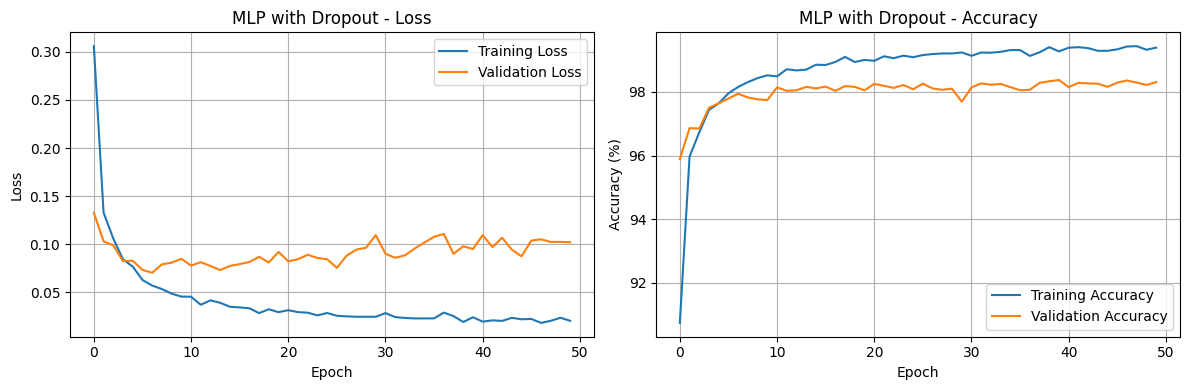
\includegraphics[width=0.7\linewidth]{section2/dropout.png}
    \caption{Training and validation curves for MLP with Dropout}
    \label{fig:dropout}
\end{figure}

\subsubsection{Question 2.1: Did dropout help reduce overfitting?}
Yes, dropout reduced overfitting. Validation accuracy improved from 97.74\% to 98.31\%, while the train-validation gap decreased from 2.05\% to 1.08\%. Validation loss remained stable around 0.08-0.10 instead of increasing to 0.19 as in the baseline and does not show an upward trend.

\subsection{Early Stopping Experiment}

\begin{itemize}
    \item Final epoch: \textbf{11}
    \item Training accuracy: \textbf{99.56\%}
    \item Validation accuracy: \textbf{97.90\%}
    \item Patience: \textbf{5 epochs}
\end{itemize}

\begin{figure}[h]
    \centering
    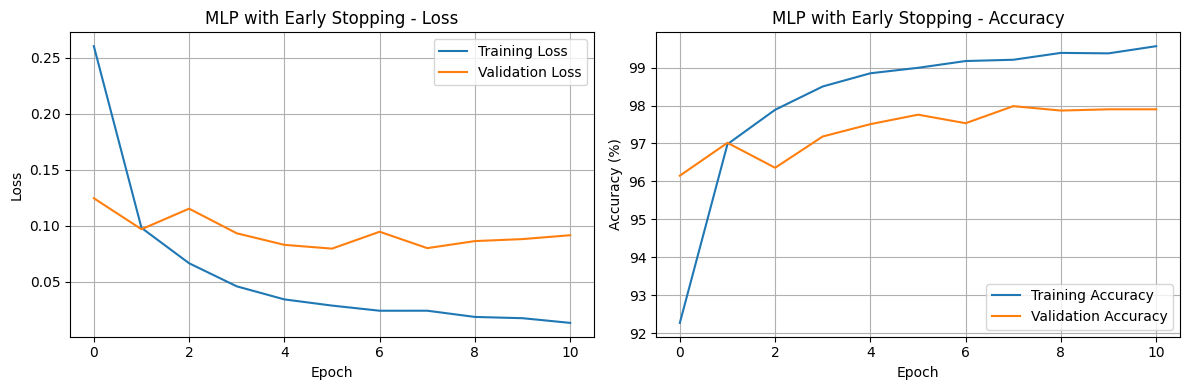
\includegraphics[width=0.7\linewidth]{section2/early_stopping.png}
    \caption{Training and validation curves for MLP with Early Stopping}
    \label{fig:early-stopping}
\end{figure}

\subsubsection{Question 2.2: How did early stopping affect performance?}
Early stopping achieved slightly better validation accuracy (97.90\% vs 97.74\%) while training for only 11 epochs instead of 50 or a 78\% reduction in training time. This shows that the baseline was over-training. Continuing beyond epoch 11 did not improve validation performance and increased overfitting.

\subsection{Regularization Comparison}

\begin{table}[h]
\centering
\begin{tabular}{|l|c|c|c|}
\hline
\textbf{Method} & \textbf{Train Acc} & \textbf{Val Acc} & \textbf{Overfitting?} \\ \hline
Baseline & 99.79\% & 97.74\% & Yes (2.05\% gap) \\ \hline
Dropout & 99.39\% & 98.31\% & No (1.08\% gap) \\ \hline
Early Stopping & 99.56\% & 97.90\% & No (stopped early) \\ \hline
\end{tabular}
\caption{Comparison of regularization techniques}
\label{tab:regularization}
\end{table}

\textbf{Conclusion:} Dropout achieved the highest validation accuracy (98.31\%) with minimal overfitting. Early stopping provided similar performance with 78\% fewer epochs making it the best choice from a computation standpoint.